\documentclass[12pt]{article}
\usepackage{amssymb}
\usepackage{scrextend}
\usepackage[utf8]{inputenc}
\usepackage[polish]{babel}
\usepackage{indentfirst}
\usepackage[T1]{fontenc}
\usepackage[utf8]{inputenc}
\usepackage{geometry}
\usepackage{float}
\usepackage{enumitem}
\usepackage{hyperref}
\usepackage{tabulary}
\usepackage{etoc}
\usepackage[normalem]{ulem} 
\usepackage{tikz}
\usepackage[bf]{caption}
\usepackage{dirtytalk}
\usepackage{listings}
\usepackage{xcolor}

\newcommand\todo[1]{\textcolor{red}{#1}}

\usepackage{graphicx}
\graphicspath{ {img/} }
\newgeometry{lmargin=2.0cm, rmargin=2.0cm, tmargin=2.0cm, bmargin=2.0cm}

\renewcommand{\baselinestretch}{1.5}
\newcommand{\paragraphnewline}[1]{\paragraph{#1}\mbox{}\\}

\bibliographystyle{ieeetr}

\definecolor{codegreen}{rgb}{0,0.6,0}
\definecolor{codegray}{rgb}{0.5,0.5,0.5}
\definecolor{codepurple}{rgb}{0.58,0,0.82}
\definecolor{backcolour}{rgb}{0.95,0.95,0.92}

\lstdefinelanguage{JavaScript}{
  morekeywords=[1]{break, continue, delete, else, for, function, if, in,
    new, return, this, typeof, var, void, while, with, import, from, as, readonly, string, export, class, async, implements},
  % Literals, primitive types, and reference types.
  morekeywords=[2]{false, null, true, boolean, number, undefined,
    Array, Boolean, Date, Math, Number, String, Object, Promise},
  % Built-ins.
  morekeywords=[3]{eval, parseInt, parseFloat, escape, unescape},
  sensitive,
  morecomment=[s]{/*}{*/},
  morecomment=[l]//,
  morecomment=[s]{/**}{*/}, % JavaDoc style comments
  morestring=[b]',
  morestring=[b]"
}[keywords, comments, strings]

\lstdefinestyle{mystyle}{
    backgroundcolor=\color{backcolour},   
    commentstyle=\color{codegreen},
    keywordstyle=\color{magenta},
    numberstyle=\tiny\color{codegray},
    stringstyle=\color{codepurple},
    basicstyle=\ttfamily\footnotesize,
    breakatwhitespace=false,         
    breaklines=true,                 
    captionpos=b,                    
    keepspaces=true,                 
    numbers=left,                    
    numbersep=5pt,                  
    showspaces=false,                
    showstringspaces=false,
    showtabs=false,                  
    tabsize=2
}
\renewcommand{\lstlistlistingname}{Spis listingów}\lstset{style=mystyle}

\widowpenalty 10000
\clubpenalty 10000

\begin{document}

% Titlepage

\begin{titlepage} % Suppresses displaying the page number on the title page and the subsequent page counts as page 1
	\newcommand{\HRule}{\rule{\linewidth}{0.5mm}} % Defines a~new command for horizontal lines, change thickness here

	\center % Centre everything on the page

	%------------------------------------------------
	%	Headings
	%------------------------------------------------

	\textsc{\LARGE Politechnika Wrocławska}\\[1.5cm] % Main heading such as the name of your university/college

	\textsc{\Large }\\[0.5cm] % Major heading such as course name

	\textsc{\large Akceleracja obliczeń w~przetwarzaniu danych}\\[0.5cm] % Minor heading such as course title

	%------------------------------------------------
	%	Title
	%------------------------------------------------

	\HRule\\[0.4cm]

	{\Huge\bfseries Wyszukiwanie podciągu w~ciągu znaków \par}% Title of your document
	\vspace{0.4cm}
	\HRule\\[1.5cm]

	%------------------------------------------------
	%	Author(s)
	%------------------------------------------------

	\begin{minipage}{0.4\textwidth}
		\begin{flushleft}
			\large
			\textit{Autorzy}\\
			Maja Bojarska, \textsc{241287} \\
			Damian Koper, \textsc{241292} \\
			Jakub Plona, \textsc{241284} \\
			Jakub Grzybek, \textsc{241365} \\
		\end{flushleft}
	\end{minipage}
	~
	\begin{minipage}{0.4\textwidth}
		\begin{flushright}
			\large \textit{Prowadzący}\\
			dr inż. Marek Woda % Supervisor's name
		\end{flushright}
	\end{minipage}

	% If you don't want a~supervisor, uncomment the two lines below and comment the code above
	%{\large\textit{Author}}\\
	%John \textsc{Smith} % Your name

	%------------------------------------------------
	%	Logo
	%------------------------------------------------

	\vfill\vfill
	% 	\includegraphics[width=0.5\textwidth]{sierpinski/opengl_logo.png}\\[2cm]

	%------------------------------------------------
	%	Date
	%------------------------------------------------

	\vfill\vfill\vfill % Position the date 3/4 down the remaining page

	{\large \today} % Date, change the \today to a~set date if you want to be precise

	\vfill % Push the date up 1/4 of the remaining page

\end{titlepage}

% TOC
\clearpage
\setcounter{tocdepth}{2}
\localtableofcontents
\listoffigures
% \lstlistoflistings

% Parts
\clearpage

\section{Wstęp}
% Kuba2
% - filozoficzne pierdoły o~akceleracji, czemu ważne blabla
% Tutaj napisz może coś o~bioinformatyce, sekwencjonowaniu dna - bo fajne i~nauka go BRRRRRR ACTGACTGACTGACTG.

\subsection{Cele i~zakres projektu}
Głównym celem tego projektu była próba akceleracji algorytmu wyszukiwania podciągu w~ciągu znaków poprzez zrównoleglenie jego składowych z~wykorzystaniem akceleratora graficznego. Za punkt odniesienia przyjęto sekwencyjną wersję algorytmu uruchamianą na CPU. Dodatkowo zbadana została zrównoleglona wersja algorytmu na dostępnych rdzeniach CPU. Do wykonania zadania akceleracji niezbędne było zdobycie informacji o~sposobie implementacji algorytmów równoległych dla GPU, gdyż ich struktura różni się od struktury standardowych \mbox{algorytmów sekwencyjnych.}

Ponadto, w~celach zawarło się wykorzystanie frameworka GPU.js, który dostarcza interfejs programistyczny pozwalający na interakcję z~procesorem graficznym w~celu wykonania standardowych obliczeń nie wpisujących się w potok graficzny. Wykorzystanie wspomnianego frameworka narzuciło uruchamianie projektu w~środowisku przeglądarki internetowej. Projekt zakładał wykorzystanie więcej niż jednej przeglądarki na więcej niż jednej platformie sprzętowej.

Zakres projektu wiąże się z~wyznaczonymi celami. Zaimplementowane zostały 3 wersje algorytmu wyszukiwania podciągu w~ciągu znaków:
\begin{itemize}[noitemsep]
    \item sekwencyjny dla CPU,
    \item równoległy dla CPU,
    \item równoległy dla GPU.
\end{itemize}
Do implementacji równoległego algorytmu dla CPU wykorzystano w~znacznym stopniu implementację sekwencyjną -- w~obu przypadkach zastosowano obecny w~przeglądarkach mechanizm workerów. Implementacja dla GPU poprzedzona została analizą algorytmu sekwencyjnego oraz wyodrębnieniem elementów dających się zrównoleglić.

Przygotowany został interfejs użytkownika pozwalający na łatwe dostosowywanie parametrów działania algorytmów, ich uruchamianie oraz pomiar czasów wykonania w~funkcji rozmiaru problemu. Posiadając tak przygotowany interfejs przeprowadzono eksperymenty oraz wyeksportowano dane pozwalające na porównanie oraz ocenę efektywności zaimplementowanych wersji algorytmu wyszukiwania ciągu znaków w~dostarczanym tekście.


\subsection{Aktualny stan wiedzy o~problemie}
Wyszukiwanie wzorca (podciągu) w~tekście (ciągu znaków) jest powszechnie występującym problemem w~dziedzinie przetwarzania tekstu. Może on zostać zdefiniowany w~następujący sposób: dla danego tekstu $ T[1..n]$ i~wzorca $ W[1..m] $, znajdź wszystkie pozycje $i$, dla których zachodzi $ T[i+k] = W[k] $, przy założeniach $ m \leq n \wedge 1 \leq k \leq m \wedge 0 \leq i~\leq n - m$.

Wcześniejsze badania wykazały, że akceleracja z~wykorzystaniem procesora graficznego ogólnego przeznaczenia (dalej zwanym GPGPU\footnote{Z ang. "general purpose graphics processing unit".}) umożliwia nawet dwudziestokrotne przyspieszenie, względem implementacji na CPU\cite{StringMatchingMulticoreGPU}. Wynik ten jest jednak zależny od czynników takich jak: długość tekstu, długość wzorca, zastosowany algorytm, model CPU i~GPGPU.

\subsection{Znane rozwiązania}
Do opisu algorytmów przyjęto, że długość przeszukiwanego tekstu wynosi $n$, natomiast długość wyszukiwanego wzorca $m$.

\begin{itemize}
    \item Metoda naiwna, znana również jako ,,brute force''. Jest prosta i~jednocześnie najmniej wydajna. Polega na przesuwaniu okna o~długości wzorca, wdłuż przeszukiwanego tekstu. Na każdej pozycji, sprawdzane jest dopasowanie wzorca do fragmentu tekstu objętego oknem\cite{NaiveSearchAlgo}. Algorytm ten ma średnią złożoność obliczeniową $\Theta(n+m)$, natomiast pesymistyczną $\mathcal{O}(nm)$. Ze względu na to, że nie wykonuje wstępnego przetwarzania danych, nie wymaga alokowania dodatkowej pamięci.
    \item Algorytm Knutha-Morrisa-Pratta wykorzystuje wiedzę na temat wyszukiwanego wzorca, na podstawie której wyznacza kolejne pozycje porównywania w~tekście\cite{KnuthMorrisPrattAlgo}. W~ten sposób, redukuje liczbę wykonywanych porównań, osiągając złożoność obliczeniową $\mathcal{O}(n)$. Dodatkowo, wymaga wstępnego przetworzenia wzorca, co obarczone jest złożonością obliczeniową i\linebreak pamięciową $\mathcal{O}(m)$.
    \item Algorytm Boyera-Moorea, w~przeciwieństwie do wyżej opisanych, sprawdza dopasowanie wzorca od jego ostatniego ($wzorzec[m]$), do pierwszego znaku ($wzorzec[1]$). W~sytuacji niedopasowania na obecnej pozycji, wykonywany jest skok, którego długość określana jest na podstawie wyniku wcześniejszego przetworzenia wzorca\cite{BoyerMooreAlgo}. Szybkość działania algorytmu wzrasta wraz ze wzrostem długości wzorca, ponieważ umożliwia to potencjalnie dłuższe skoki. Pesymistyczna złożoność obliczeniowa przetwarzania wstępnego wynosi $\mathcal{O}(m)$, a~wyszukiwania $\mathcal{O}(mn)$. Pamięć wymagana do przechowania wyniku wstępnego przetworzenia wzorca wynosi $\Theta(k)$, gdzie $k$ stanowi długość alfabetu (zbioru znaków) wykorzystanego w~tekście.
    \item Algorytm Rabina-Karpa wykorzystuje funkcję skrótu (ang. hash function) do wstępnej oceny dopasowania wzorca\cite{RabinKarpAlgo}. Jego wydajność jest zależna od wybranej funkcji skrótu, której obliczenie nie powinno być kosztowne. Wyszukiwanie wzorca polega na porównywaniu skrótu wzorca $hash(wzorzec[1..m])$, do skrótu fragmentu tekstu $hash(tekst[i..i+m-1])$, dla $1 \leq i~\leq n-m+1$. Równość skrótów w~ogólnym przypadku nie gwarantuje dopasowania ciągów znaków, dla których zostały obliczone. Dlatego, aby móc stwierdzić wykrycie wzorca, należy dodatkowo porównać ciągi znaków.
    Algorytm ten stanowi dobre rozwiązanie dla problemu wyszukiwania wielu (różnych) wzorców w~tekście. Jego złożoność zależy od wykorzystanej funkcji skrótu. W~kontekście wyszukiwania pojedynczego wzorca, jest mniej wydajny od algorytmów Boyera-Moorea i~Knutha-Morrisa-Pratta. 

\end{itemize}


\section{Model systemu}

\subsection{Wybrany wariant problemu}

Do realizacji projektu wybrany został problem w~wariancie wyszukiwania dokładnego, za pomocą metody naiwnej. Powodem tej decyzji jest łatwość zrównoleglenia algorytmu, zarówno dla wielowątkowej implementacji na CPU, jak i~dla GPGPU.

Metryką wybraną do oceny jakości zaimplementowanego rozwiązania jest akceleracja, uzyskana z~wykorzystania GPGPU. Wynika ona ze stosunku czasów rozwiązania problemu na GPGPU, do CPU. Została opisana wzorem~\ref{SpeedupRatio}.

\begin{equation}
    \label{SpeedupRatio}
    S=\frac{T_{GPGPU}}{T_{CPU}}
\end{equation}

Zakłada się, że badane rozwiązania przyjmują zadaną instancję problemu (tekst i~wzorzec), a~następnie zwracają wynik działania w~postaci zbioru liczb, będących pozycjami wystąpień wzorca w~tekście. Wygenerowanie instancji problemu, wykorzystywanej do testów, nie jest wliczane w~mierzony czas rozwiązania.

\subsection{Projekt i~implementacja systemu}

Projekt, w~swoich założeniach mając testować możliwości akceleracji omawianego problemu w~środowisku przeglądarki internetowej, wymusił zaimplementowanie wszystkich elementów systemu w~tymże środowisku. Separacja części systemu o~różnej odpowiedzialności pozwoliła rozwijać je niezależnie od siebie.
Wyodrębniono domeny odpowiedzialne za pomiar wydajności testowanych rozwiązań, algorytmy wykonywane na CPU i~GPU, generowanie danych testowych oraz \mbox{interfejs użytkownika.}

\subsubsection{Narzędzia i~technologie}

System dla użytkownika widoczny jest jako strona internetowa typu Single Page Application, umożliwiająca przetestowanie zdefiniowanego problemu na różnych przeglądarkach internetowych i~maszynach o~różnej konfiguracji sprzętowej. Całość budowana jest przy pomocy narzędzia Webpack~\cite{Webpack}. Za funkcjonowanie interfejsu użytkownika odpowiada framework React~\cite{React}, a~za interaktywne wykresy framework Plotly.js~\cite{Plotly}.

Pomiar wydajności pierwotnie korzystać miał z~biblioteki benchmark.js, lecz jego niekompatybilność z~systemem budowania projektu wymusiła stworzenie znacznie prostszego systemu pomiaru czasu. Stworzony system pomiarowy korzysta z~interfejsu \texttt{Performance}~\cite{HRT} przeglądarki i~pozwala na wielokrotne powtórzenie testu dla tych samych danych. Na podstawie powtórzeń wyliczone zostają statystyki powiązane z~testowanym rozmiarem problemu.

Rozmiar rozwiązywanego problemu opisany jest jako rozmiar wzorca oraz rozmiar przeszukiwanego tekstu. Oba ciągi znaków generowane za pomocą liczb pseudolosowych i~konwertowane są do postaci bajtowej w~tablicy typu \texttt{Uint8Array} za pomocą interfejsu \texttt{TextEncoder} \cite{TextEncoder}. Wszystkie tablice korzystają ze współdzielonych buforów pamięci \texttt{SharedArrayBuffer}, co umożliwia uniknięcie opóźnień wynikających z~kopiowania pamięci.

Algorytm rozwiązujący problem na CPU korzysta z~mechanizmu Workerów. Pozwala definiować ich liczbę, która odpowiada stopniowi zrównoleglenia obliczeń. Obliczenia na GPU korzystają z~API WebGL2, którego nadrzędnym celem jest generowanie grafiki 2D i~3D. Odpowiednio interpretując wynikowe wartości przetwarzania danych wejściowych jesteśmy w~stanie użyć jej do obliczeń niemających nic wspólnego z~grafiką. Biblioteką użytą i~stanowiącą warstwę abstrakcji pomiędzy WebGL, a~prowadzeniem obliczeń jest GPU.js~\cite{GPU.js}.

\subsubsection{Algorytmy}
% Maja
% - abstrakcyjny scheduler i~wspólny interface
% - odniesienia do UMLi, class D
% - UMLe bardzo pływające, niech latex sobie ułoży sam
% - ważny taki ram format wyjściowy (dla analizy GPU) - tablica wystąpień

Klasą bazową, która zarządza konkretnym rozwiązaniem i~harmonogramuje jego uruchomienie, jest \texttt{CoreScheduler}. Ustala on również oczekiwany interfejs wejścia dla instancji problemu\linebreak (\texttt{DataInMessageBasePayload}) i~interfejs wyjścia dla wyniku (\texttt{DataOutMessageBasePayload}).\linebreak Zakłada się, że wynik jest zawsze podawany w~postaci zbioru liczb, określających pozycje w~tekście, na których wykryto wzorzec. \texttt{DataProvider} ułatwia generowanie pseudolosowych instancji problemu o~określonej długości tekstu i~wzorca, w~formacie oczekiwanym przez \texttt{CoreScheduler}.

Rozmiar problemu oraz liczba wątków rozwiązujących problem określana jest przez użytkownika, za pośrednictwem interfejsu graficznego aplikacji. Po rozpoczęciu testu dla zadanej konfiguracji, generowana jest instancja problemu za pomocą klasy \texttt{DataProvider}.

Poniżej opisane zostało działanie dwóch wariantów algorytmu, które ma miejsce bezpośrednio pomiędzy rozpoczęciem i~zakończeniem pomiaru czasu.

\begin{figure}
    \centering
    \includegraphics[keepaspectratio, width=1.0\linewidth]{diagrams/out/core_class.png}
    \caption{Diagram klas bazowych.}
    \label{DiagramClassCPU}
\end{figure}

\paragraph{Wersja dla CPU}
% Maja & Damian
% - ustawienie concurrency
% - workery nie są od razu ready - są łądowane asynchronicznie
% - pierwsze wykonanie nieco wolniejsze, optymalizacja JIT silnika (chyba)
% - ^- to już przy analizie wydajności
% - opisanie właściwego algorytmu
% - odniesienia do UMLi, sequence D

W wariancie algorytmu wykonywanym na CPU, instancja problemu wraz z~oczekiwaną liczbą procesów go rozwiązujących przekazywana jest do \texttt{CpuScheduler}, który przygotowuje odpowiednią liczbę instancji klasy \texttt{CpuSolver} i~zarządza ich uruchomieniem. Każda z~instancji \texttt{CpuSolver}, funkcjonuje jako osobny Worker, co umożliwia ich współbieżne działanie i~wykorzystanie wielu rdzeni procesora \cite{WebWorker}. Po rozwiązaniu wydzielonej części problemu, każdy \texttt{CpuSolver} zwraca uzyskane wyniki. Następnie, \texttt{CpuScheduler} agreguje wyniki częściowe i~zwraca je do interfejsu graficznego. Całkowity czas rozwiązania problemu jest mierzony i~przedstawiany użytkownikowi.
Strukturę klas implementujących rozwiązanie na CPU przedstawia diagram \ref{DiagramClassCPU}, natomiast sekwencję ich działań, diagram \ref{DiagramSequenceCPU}.

Workery, w~związku ze specyfiką swojego funkcjonowania, muszą być ładowane asynchronicznie -- ich kod pobierany jest osobnym zapytaniem do serwera. Wprowadza to opóźnienie związane z~tworzeniem i~usuwaniem workerów. Nie było jednak ono brane pod uwagę podczas pomiarów wydajności. Przed rozpoczęciem pomiarów następuje synchronizacja wszystkich workerów.


\begin{figure}
    \centering
    \includegraphics[keepaspectratio, width=1.0\linewidth]{diagrams/out/cpu_class.png}
    \caption{Diagram klas rozwiązania na CPU.}
    \label{DiagramClassCPU}
\end{figure}

\begin{figure}
    \centering
    \includegraphics[keepaspectratio, width=1.0\linewidth]{diagrams/out/cpu_sequence.png}
    \caption{Diagram sekwencji rozwiązania na CPU.}
    \label{DiagramSequenceCPU}
\end{figure}


\paragraph{Wersja dla GPU}
% Kuba & Damian
% - ustawienie concurrency - zawsze 1 optymalizacja pod względem obciążenia GPU, maksymalizacja liczby kerneli [+/-]
% - wszystko synchronicznie - od razu ready [-]
% - pierwsze wykonanie wolniejsze, optymalizacja JIT silnika (chyba) budowanie kernela, później kernel keszowany [+/-]
% - opisanie właściwego algorytmu [+]
% - odniesienia do UMLi, sequence D [+]

% Damian - tutaj o~schedulerze + pomiar czasu + jakieś połączenie z~dalszym tekstem

Analogicznie jak w~przypadku algorytmu na CPU, klasą zarządzającą wykonaniem obliczeń jest klasa rozszerzająca klasę \texttt{CoreScheduler} -- \texttt{GpuScheduler}. Wykonanie tego wariantu algorytmu nie odbywa się asynchronicznie i~blokuje wątek główny przeglądarki, co oznacza, że dalsza synchronizacja nie jest wymagana. \texttt{GpuScheduler} tworzy i~zarządza instancją klasy \texttt{GpuSolver}, która bezpośrednio korzysta z~biblioteki GPU.js, pozwalającą na wykonywanie obliczeń bezpośrednio na GPU poprzez abstrakcję kernela.

Szczegóły struktur zdefiniowanych klas oraz interfejsów można znaleźć na diagramie klas~\ref{DiagramClassGPU}. Sekwencje operacji logicznych systemu, odpowiedzialnych za obsługę żądania wykonania algorytmu na GPU są przedstawione na diagramie sekwencji~\ref{DiagramSequenceGPU}.

\begin{figure}
    \centering
    \includegraphics[keepaspectratio, width=1.0\linewidth]{diagrams/out/gpu_class.png}
    \caption{Diagram klas rozwiązania na GPU.}
    \label{DiagramClassGPU}
\end{figure}

\begin{figure}
    \centering
    \includegraphics[keepaspectratio, width=1.0\linewidth]{diagrams/out/gpu_sequence.png}
    \caption{Diagram sekwencji rozwiązania na GPU.}
    \label{DiagramSequenceGPU}
\end{figure}

\begin{samepage}

    Przed wykonaniem obliczeń, w~klasie \texttt{GpuSolver}, dane wejściowe algorytmu są sprawdzane pod kątem błędów. Wyznaczone niedozwolone przypadki to:
    \begin{itemize}[noitemsep]
        \item tekst pusty,
        \item wzorzec pusty,
        \item wzorzec dłuższy od tekstu.
    \end{itemize}
\end{samepage}

Jeżeli spełniony zostanie co najmniej jeden z~wymienionych warunków, obliczenia nie są wykonywane, zaś algorytm zwraca odpowiedź bez rozwiązania z~odpowiednią informacją o~błędzie. W~przeciwnym wypadku wykonywane są wstępne obliczenia na CPU przygotowujące strukturę kernela dla GPU.

Wymaganiem nałożonym na etap wstępnych obliczeń jest możliwie szybkie jego wykonanie. Z~uwagi na przyjęty sposób przydziału podproblemów wyszukiwania do wątków karty graficznej, szerzej opisany w~następnych akapitach, implementacja tego etapu charakteryzuje się złożonością $\mathcal{O}(1)$. Wykonywane jest tutaj jedynie odejmowanie długości wzorca od długości tekstu wyznaczające liczbę pozycji bazowych do porównań tekstu i~wzorca (tzw. okien), które zostaną rozdzielone pomiędzy wątki uruchamiane na GPU.

Do kompilacji kernela potrzebna jest informacja o~formacie danych wyjściowych z~GPU, którą na tym etapie algorytm posiada. W~celach optymalizacyjnych kompilacja wykonywana jest tylko wtedy, gdy jest to konieczne. Algorytm sprawdza, czy zmienił się format wyjścia danych z~GPU (liczba okien, tj. liczba wątków) i~jeżeli nie nastąpiła taka zmiana, to wykorzystywana jest przechowywana, wcześniej skompilowana wersja kernela.

Sam algorytm dla pojedynczego wątku GPU jest możliwie prosty. Wykonywane jest porównanie wzorca z~tekstem na pozycji wyznaczonej przez numer wątku; wątków logicznych jest tyle samo, co okien. Porównanie to jest wykonywane w~pętli, gdzie liczba iteracji jest ograniczona z~góry przez długość wzorca. Wątek obliczeniowy GPU zwraca $-1$, jeżeli okaże się, że i-ta pozycja wzorca jest różna od odpowiadającej jej pozycji w~tekście. Jeżeli wzorzec i~tekst są równe w~n-tym oknie, którego indeks jest jednocześnie indeksem wątku, to zwracany jest właśnie ten indeks.

Przyjęto, iż ogólny format danych wyjściowych z~algorytmu wyszukiwania będzie miał strukturę listy z~indeksami, na których wystąpiło dopasowanie -- jest to struktura gęsta (,,dense''). Niestety format danych wyjściowych z~GPU ma z~góry narzuconą strukturę rzadką (,,sparse'') -- lista zawiera wynik dla każdego zbadanego okna. Wymusza to dodatkową konwersję wyjścia GPU do formatu gęstego. Operacja ta jest wykonywana przez CPU ze złożonością $\mathcal{O}(n)$. Po konwersji danych wyjściowych GPU, algorytm jest gotowy do zwrócenia wyniku.

% Damian - tutaj o~odebraniu wyniku i~zakończeniu pomiaru czasu
Dane wejściowe dobrane są tak, że gwarantują co najmniej jedno wykrycie wzorca w~tekście. Ze względu na specyfikę pomiarów wydajności, wynik nie jest nigdzie przechowywany, a~referencja do wynikowej tablicy zostaje finalnie usunięta przez mechanizm Garbage Collector.


\subsection{Interfejs użytkownika}
% Kuba2 & Damian
% - react
% - wykresy Plotly, 
% - konfiguracja uruchamiania, warianty 
% - jak zrobić co (np generujemy serię, klikamy na punkt i~wyświetla się histogram)

Interfejs przygotowano w formie panelu webowego z~pomocą biblioteki \emph{React}. Do dyspozycji użytkownika oddano zestaw narzędzi, który pozwala na konfigurację parametrów testowanego algorytmu oraz przeglądanie wyników jego działania w~postaci wykresów i~histogramów. 

Panel dzieli się na dwie główne części. Pierwsza, górna, pozwala na wprowadzenie podstawowych wartości konfiguracyjnych dla algorytmu takich, jak długość badanego tekstu i~długość poszukiwanego wzorca, oraz parametry określające jak zwiększać mają się wspomniane wartości z~kolejnymi testami. Dodatkowo w~pierwszej części interfejsu użytkownik ma możliwość sprawdzenia specyfikacji systemu, przeglądarki oraz komputera na jakim uruchomione jest oprogramowanie. 

Druga część interfejsu przeznaczona jest do wykonywania testów i~podglądu wyników ich działania. Dzieli ona się na cztery zakładki: trzy dla różnych wariantów badanego algorytmu oraz czwarta pozwalająca na podgląd podsumowania wykonanych testów. W~poszczególnych zakładkach zdefiniować można dodatkowo parametry dla danego wariantu algorytmu takie, jak ilość powtórzeń każdego problemu lub ilość wątków bądź kerneli w~przypadku algorytmów wielowątkowych. 

Przy wykonywaniu badań użytkownik ma dostęp do kilku wykresów. Pierwszy z~nich oferuje dostęp do średniego czasu wykonania algorytmu w~zależności od długości problemu. Dodatkowo na wykresie zaznaczane jest odchylenie standardowe, minimum i~maksimum dla każdego z~punktów. Na kolejnych wykresach użytkownik może obserwować konkretne wartości z~badań, takie, jak maksymalny oraz minimalny czas wykonania oraz jego wariancja i~odchylenie standardowe. 

Do wyświetlenia wykresów wykorzystano bibliotekę \emph{Plotly.js}. Oferuje ona bardzo duży zakres możliwości i~personalizacji.  W~ramach \emph{Plotly.js} dostarczane jest ponad 40 typów wykresów w~tym między innymi wykresy 3D i~mapy. W~przygotowaniu omawianego panelu wykorzystano zaplecze do tworzenia grafów statystycznych. Oprogramowanie oferuje między innymi możliwość wyboru wyświetlanych zestawów danych, przybliżania czy zapisywania wykresów w~formie obrazów PNG, co gwarantuje dużą wygodę w~analizie wyników badań.


% Nie dawajcie [ht] tylko odwołajcie się \ref w~opisie to latex to sam ładnie ułoży

\section{Analiza działania algorytmów}
% Wykresy Damian & Maja, opis Kuba
% Nie zapomnieć o~profilerze, skriny som jusz

W ramach pomiarów wydajności przeprowadzono testy na dwóch przeglądarkach, z wykorzystaniem dwóch platform sprzętowych. Z~racji na podobieństwa niektórych wyników, nie wszystkie dane opisujące różne warianty wykonania algorytmów zostały zaprezentowane w~dalszych opisach. Zwrócono jednak uwagę na istotne różnice. W~tabeli~\ref{tab:1} przedstawiono używane konfiguracje zestawów pomiarowych, do których odnosić się będą późniejszy opisy. Rozmiarem problemu jest długość przeszukiwanego tekstu. Długość wzorca jest zawsze równa 7, czyli w~zaokrągleniu tyle, ile wynosi średnia długość wyrazu w~języku polskim~\cite{Polski}. Każda seria danych wykresu średniego czasu wykonania algorytmu zawiera dodatkowo czas minimalny i maksymalny w postaci pionowych linii, a także odchylenie standardowe w postaci zacieniowanego obszaru.
\begin{table}[H]
    \centering
    \begin{tabular}{ |r l l l|  }
        \hline
        Konfiguracja & CPU                               & GPU                   & Przeglądarka    \\
        \hline
        \hline
        1.1          & Intel Core i7-4770S CPU @ 3.10GHz & Nvidia GTX 970        & Google Chrome   \\
        1.2          & Intel Core i7-4770S CPU @ 3.10GHz & Nvidia GTX 970        & Mozilla Firefox \\
        2.1          & Intel Core i5-6300U CPU @ 2.40GHz & Intel HD Graphics 520 & Google Chrome   \\
        2.2          & Intel Core i5-6300U CPU @ 2.40GHz & Intel HD Graphics 520 & Mozilla Firefox \\
        \hline
    \end{tabular}
    \caption{Konfiguracje zestawów pomiarowych}
    \label{tab:1}
\end{table}

\subsection{Wersja dla CPU -- jeden wątek}

Pierwszym przedmiotem badania jest pomiar czasu wykonania algorytmu na jednym wątku CPU. Na rysunku \ref{fig:chart_cpu_sc_mean_chrome} przedstawiono czas wykonania przy rosnącym rozmiarze problemu. Zgodnie z oczekiwaniami, przy stałym rozmiarze wzorca, złożoność algorytmu jest liniowa.
Środowisko przeglądarki internetowej, ze względu na skupienie się na obsłudze interfejsu użytkownika i asynchronicznych zadaniach, toleruje dłuższe opóźnienia. Opóźnienia te są widoczne w postaci dużego zróżnicowania czasów maksymalnych i wynikają prawdopodobnie z asynchronicznej komunikacji pomiędzy wątkami, która nie musi mieć dużego priorytetu dla przeglądarki.

% Różnice pomiędzy przeglądarkami, napomknąć o~wielu testach

\begin{figure}
    \centering
    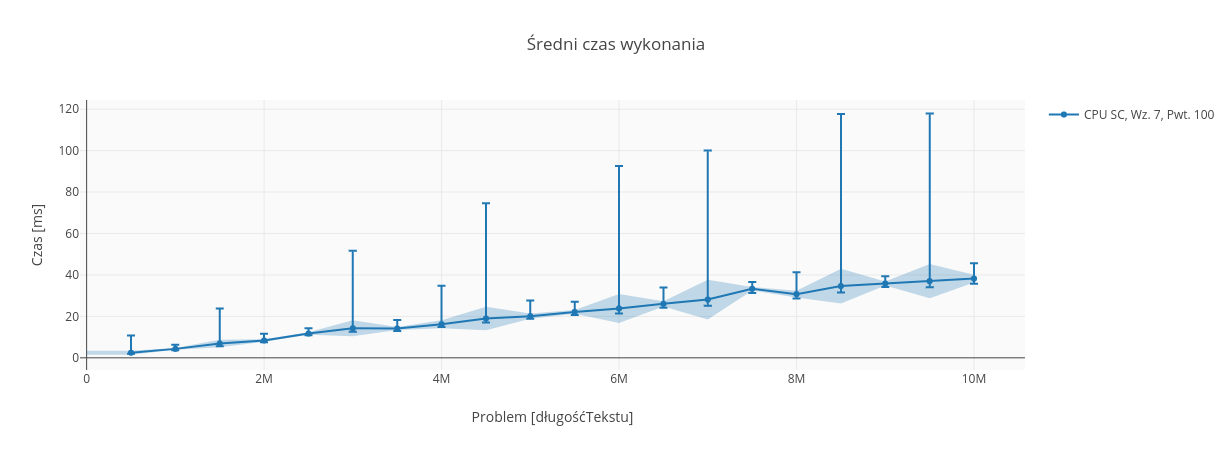
\includegraphics[keepaspectratio, width=1.0\linewidth, trim=1.1cm 0.9cm 0.5cm 3.5cm, clip]{benchmarks/nvidia970_chrome/cpu_sc_mean.png}
    \caption{Czas wykonania algorytmu CPU, jeden wątek, zestaw 1.1}
    \label{fig:chart_cpu_sc_mean_chrome}
\end{figure}


\begin{figure}
    \centering
    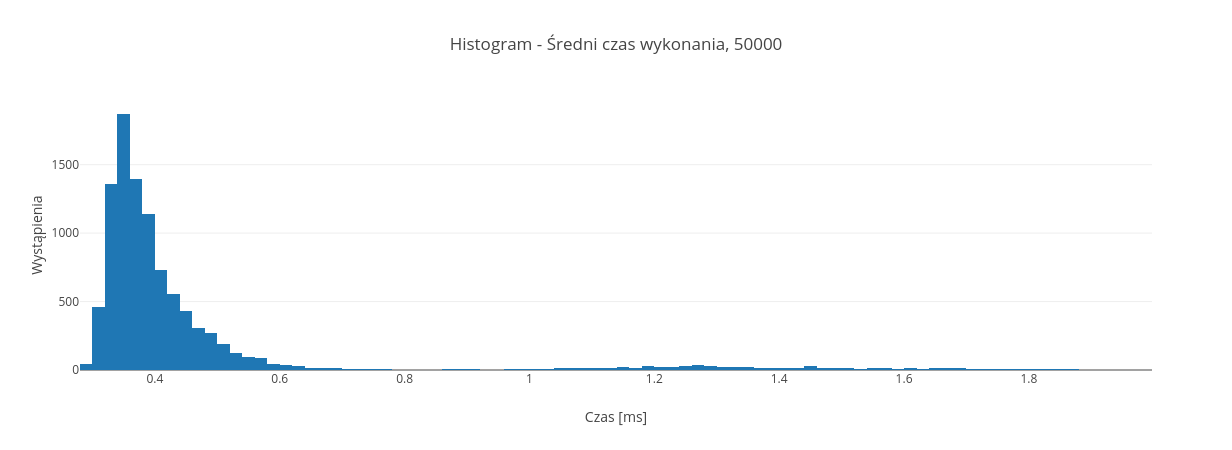
\includegraphics[keepaspectratio, width=1.0\linewidth, trim=1.1cm 0.9cm 0.5cm 3.5cm, clip]{benchmarks/nvidia970_chrome/his.png}
    \caption{Histogram czasu wykonania algorytmu CPU, problem 50.000/7, 10.000 powtórzeń, jeden wątek, zestaw 1.1}
    \label{fig:chart_cpu_sc_his_chrome}
\end{figure}

Zróżnicowanie czasu wykonania zobaczyć można dobrze na histogramie na rysunkach~\ref{fig:chart_cpu_sc_his_chrome} i~\ref{fig:chart_cpu_sc_his_firefox}. Analizując wykres dla zestawu 1.1 (Google Chrome) widać, że czas w~zdecydowanej większości oscyluje w~okolicach $0.4$~ms, ale część wyników pojawia się również w~zakresie $1.2-1.4$~ms. Przeglądarka Mozilla Firefox (rysunek~\ref{fig:chart_cpu_sc_mean_firefox} i~\ref{fig:chart_cpu_sc_his_firefox}) okazała się być mniej wydajna. Dla małych czasów wykonania istotny może być fakt, że ze względów bezpieczeństwa Mozilla Firefox ma ograniczoną precyzję pomiaru czasu z~użyciem interfejsu \texttt{Performance}.


\begin{figure}
    \centering
    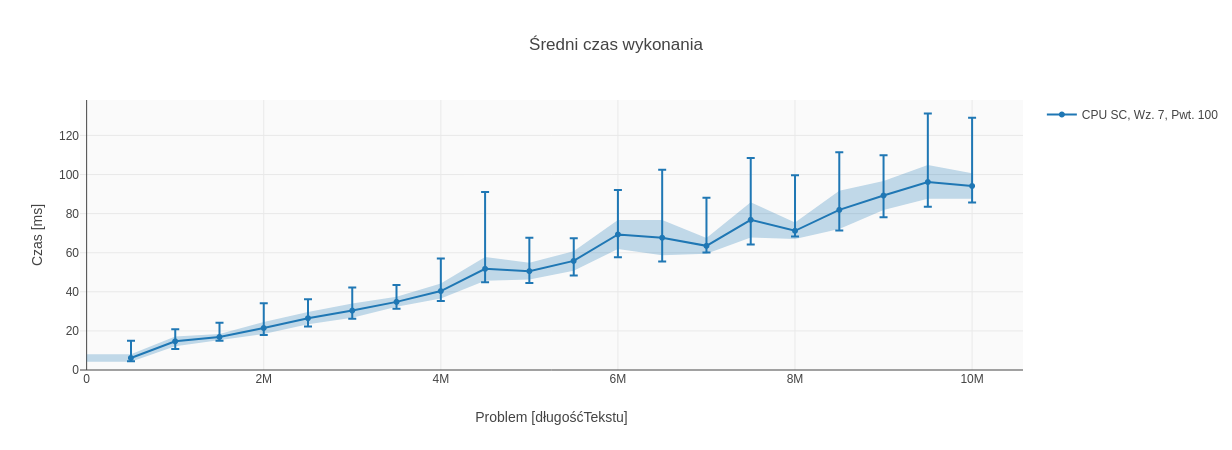
\includegraphics[keepaspectratio, width=1.0\linewidth, trim=1.1cm 0.9cm 0.5cm 3.5cm, clip]{benchmarks/nvidia970_firefox/cpu_sc_mean.png}
    \caption{Czas wykonania algorytmu CPU, jeden wątek, zestaw 1.2}
    \label{fig:chart_cpu_sc_mean_firefox}
\end{figure}

\begin{figure}
    \centering
    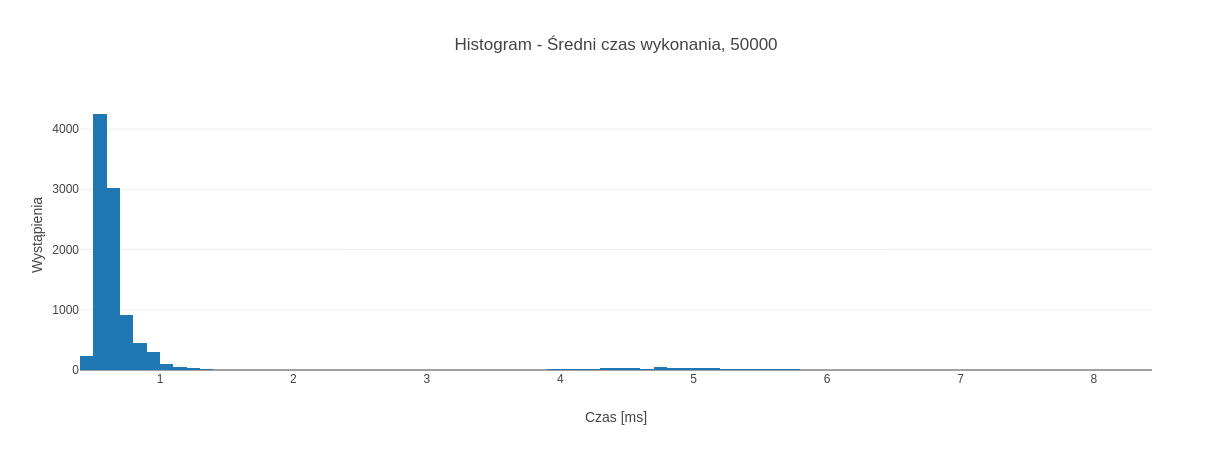
\includegraphics[keepaspectratio, width=1.0\linewidth, trim=1.1cm 0.9cm 0.5cm 3.5cm, clip]{benchmarks/nvidia970_firefox/his.png}
    \caption{Histogram czasu wykonania algorytmu CPU, problem 50.000/7, 10.000 powtórzeń, jeden wątek, zestaw 1.2}
    \label{fig:chart_cpu_sc_his_firefox}
\end{figure}

\subsection{Wersja dla CPU -- wiele wątków}
% - porównać diagramy Mai i~Damiana (2(4)Core vs 4(8)Core)

Kolejno zbadano pomiar czasu wykonania przy podziale podzadań wyszukiwania na wiele wątków. Na rysunkach~\ref{fig:chart_cpu_mc_mean_chrome_damian} i~\ref{fig:chart_cpu_mc_mean_chrome_maja} przedstawiono wyniki pomiaru czasu wykonania dla różnej liczby wątków. Zestaw 1.1 posiada czterordzeniowy CPU i na wykresie widoczne jest, że czas wykonania maleje względem wykonania jednowątkowego dla dwóch i czterech wątków. Dalsze zwiększanie liczby wątków nie przynosi przyspieszenia.
Zestaw 2.1 posiada dwurdzeniowy CPU i w tym przypadku zysk w postaci czasu wykonania widać tylko dla dwóch wątków.


\begin{figure}
    \centering
    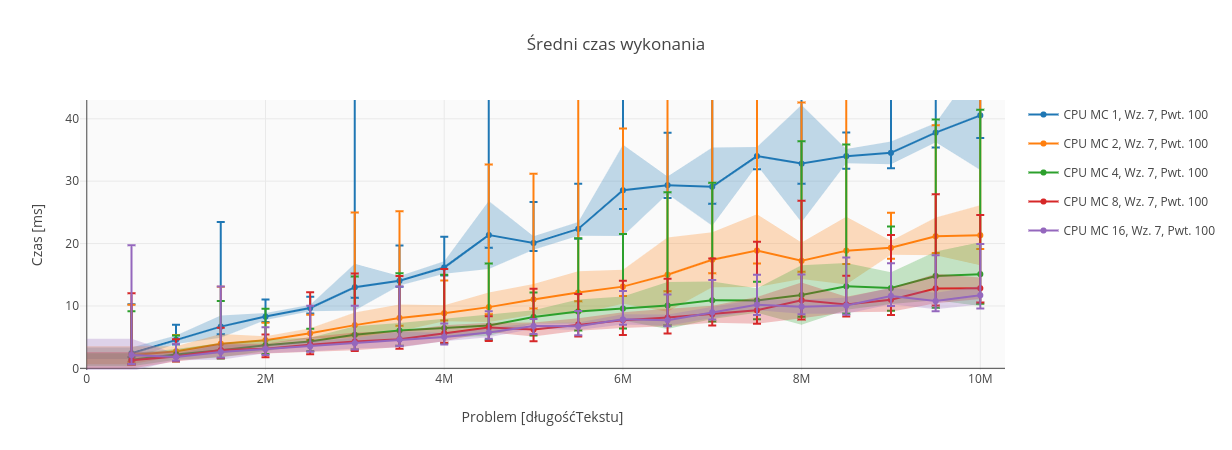
\includegraphics[keepaspectratio, width=1.0\linewidth, trim=1.1cm 0.9cm 0.5cm 3.5cm, clip]{benchmarks/nvidia970_chrome/cpu_mc_mean_zoom.png}
    \caption{Czas wykonania algorytmu CPU Multi Core, zestaw 1.1}
    \label{fig:chart_cpu_mc_mean_chrome_damian}
\end{figure}

\begin{figure}
    \centering
    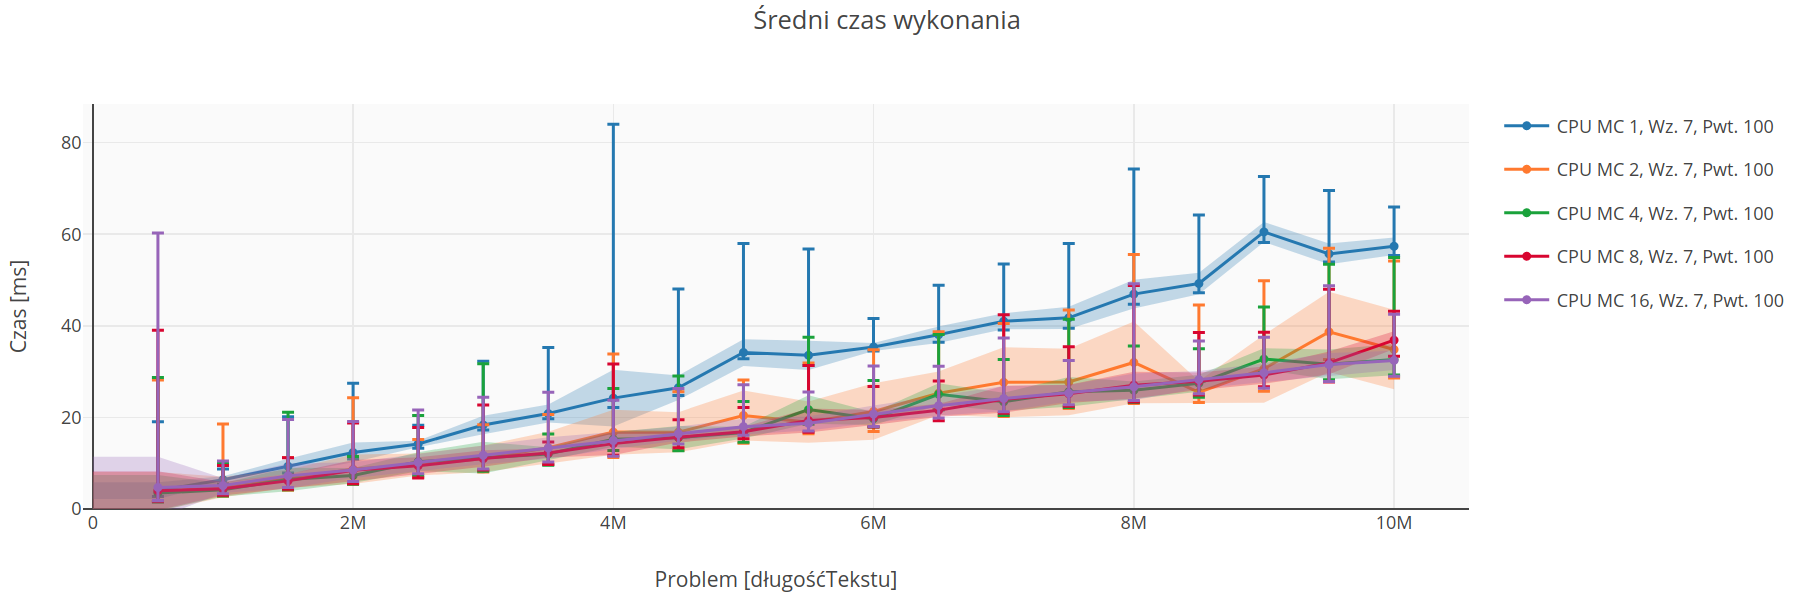
\includegraphics[keepaspectratio, width=1.0\linewidth, trim=0 0 0 2.7cm, clip]{benchmarks/intel_hd520_chrome/cpu_mc_mean.png}
    \caption{Czas wykonania algorytmu CPU Multi Core, zestaw 2.1}
    \label{fig:chart_cpu_mc_mean_chrome_maja}
\end{figure}

Na rysunku~\ref{fig:profiler_cpu} zamieszczono wycinek graficznej reprezentacji analizy profilera przeglądarki Google Chrome wykonania algorytmu na dwóch wątkach. Można zauważyć, że pierwsze wykonanie jest z reguły wolniejsze od pozostałych.

\begin{figure}
    \centering
    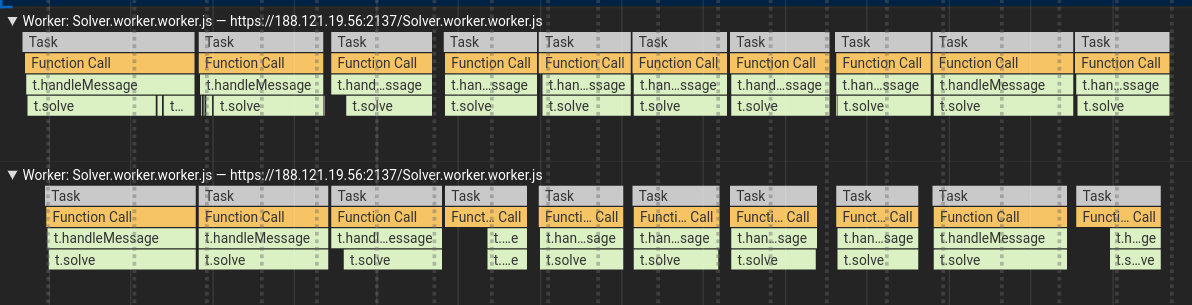
\includegraphics[keepaspectratio, width=1.0\linewidth]{benchmarks/nvidia970_chrome/cpu_2_profiler.png}
    \caption{Analiza wykonania algorytmu CPU, zestaw 1.1}
    \label{fig:profiler_cpu}
\end{figure}


\subsection{Wersja dla GPU}
% - dlaczego wyszło jak wyszło
% - rozmiar problemu rośnie razem z~wynikiem
% - tutaj dać te wzorki w~porównaniu do macierzy i~porównać do macierzy

% - dużo zajmuje pobranie wyniku
% - dużo zajmuje interpretacja wyniku (filter)


Celem w zadaniu akceleracji dla wyszukiwania wzorca (o stałej długości) w tekście, w przypadku algorytmu naiwnego jest osiągnięcie złożoności poniżej $\mathcal{O}(n)$; docelowo $\mathcal{O}(1)$ dla przypadków nie wykraczających poza możliwości karty graficznej. Niestety, jak widać na rysunkach \ref{fig:chart_gpu_mean_chrome_damian} oraz \ref{fig:chart_gpu_mean_chrome_maja} algorytm uruchomiony na GPU charakteryzuje się liniową zależnością czasu wykonania od rozmiaru problemu bez względu na konfigurację sprzętową. Tak, jak w przypadku CPU zauważalna jest niestabilność środowiska przeglądarki, co wpływa na duży rozrzut uzyskanych pomiarów czasu wykonania, jednak w przypadku GPU rozrzut tej jest zauważalnie mniejszy. Może to wynikać z faktu, iż przeglądarka nie przydziela zadań GPU tak niedeterministycznie, jak w przypadku CPU.

Ciekawy okazuje się rozkład całkowitego czasu wykonania algorytm na jego części składowe, który można zaobserwować na rysunku \ref{fig:profiler_gpu} przedstawiającym dane narzędzia profilującego wbudowanego w przeglądarkę. Jak się okazuje, kluczowy jest udział podzadań w całkowitym czasie wyszukiwania. Całkowity czas zadania z pominięciem stałych jest oznaczony na rysunku \ref{fig:profiler_gpu} jako \textit{t.solve}. Kluczowe składowe to: 
\begin{enumerate}
    \item wykonanie obliczeń na GPU - element \textit{run},
    \item odczytanie bufora GPU - element \textit{readPixels},
    \item konwersja wyjścia GPU do formatu gęstego (lista indeksów tekstu pasującego do wzorca) - czas pomiędzy zakończeniami \textit{readPixels} i \textit{t.solve}.
\end{enumerate}
Po zbadaniu danych narzędzia profilującego dla algorytmu wyszukiwania na GPU okazuje się, że elementy te mają udział w ogólnym czasie wykonania \textit{t.solve}:
\begin{itemize}
    \item dla właściwych obliczeń - 5\%,
    \item dla odczytania bufora GPU - 20\%,
    \item dla operacji przetworzenia danych wyjściowych z GPU - 75\%.
\end{itemize}
Dzieje się tak, gdyż obliczenia dla jednego wątku GPU nie są wymagające pod względem czasu. Uwidaczniają się tutaj problemy akceleracji obliczeń: gdy czas kopiowania danych jest znacznie większy od czasu wykonywanych obliczeń, trudno jest osiągnąć przyspieszenie. Dla konkretnego przypadku tego algorytmu w połączeniu z freamworkiem GPU.js, od którego zależy wymaganie czasowe funkcji \textit{readPixels()} okazuje się, iż uzyskanie akceleracji jest dodatkowo utrudnione, gdyż wyniki poszczególnych wątków są czytane sekwencyjnie. Implementacja algorytmu na GPU przydziela każdemu wątkowi GPU indeks w potencjalnie dużym tekście, co sprawia, że wyników do sekwencyjnego odczytania jest dużo -- uwidacznia się to w stosunku czasów wykonania 4:1 pomiędzy operacją odczytania wyników GPU, a właściwymi obliczeniami.

Nietrudno też zauważyć znaczną dominację czasową przetworzenia danych wynikowych z GPU przez CPU. Format wyjścia GPU jest z góry narzucony, dlatego aby uzyskać akcelerację należy zastanowić się nad koniecznością wykonywania konwersji. Jeżeli nie wymagają tego zależności zewnętrzne, konwersje wyjścia GPU powinny zostać wyeliminowane -- w przeprowadzonych badaniach konwersja taka zajęła trzykrotnie więcej czasu niż samo przetwarzanie na GPU.

\begin{figure}
    \centering
    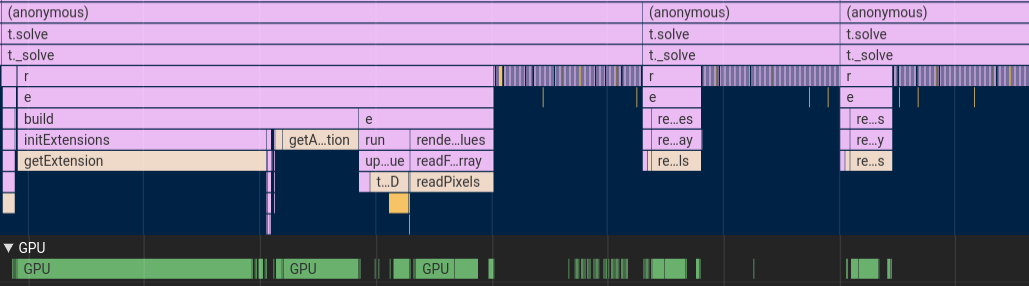
\includegraphics[keepaspectratio, width=1.0\linewidth]{benchmarks/nvidia970_chrome/gpu_profiler.png}
    \caption{Analiza wykonania algorytmu GPU, zestaw 1.1}
    \label{fig:profiler_gpu}
\end{figure}

\begin{figure}
    \centering
    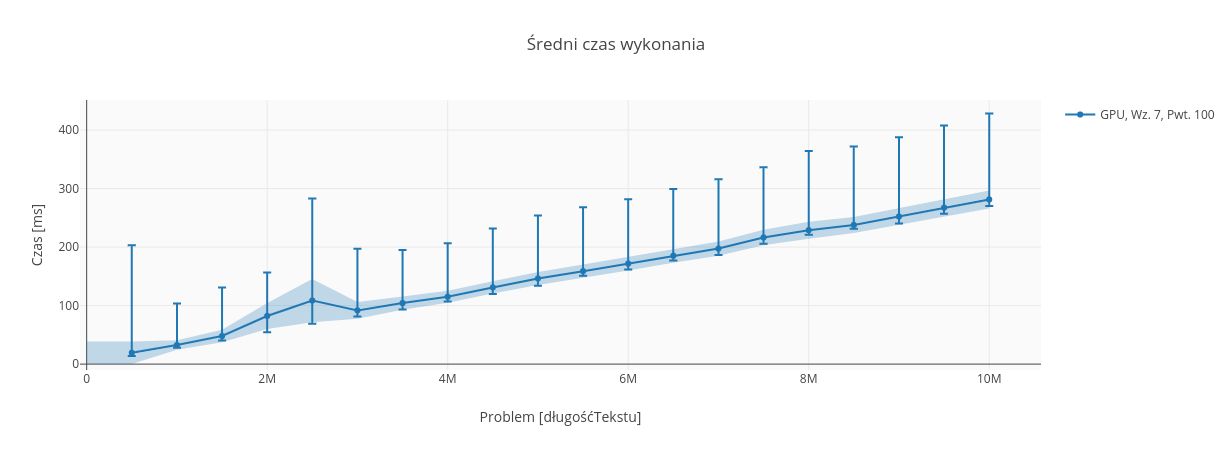
\includegraphics[keepaspectratio, width=1.0\linewidth, trim=1.1cm 0.9cm 0.5cm 3.5cm, clip]{benchmarks/nvidia970_chrome/gpu_mean.png}
    \caption{Czas wykonania algorytmu GPU, zestaw 1.1}
    \label{fig:chart_gpu_mean_chrome_damian}
\end{figure}

\begin{figure}
    \centering
    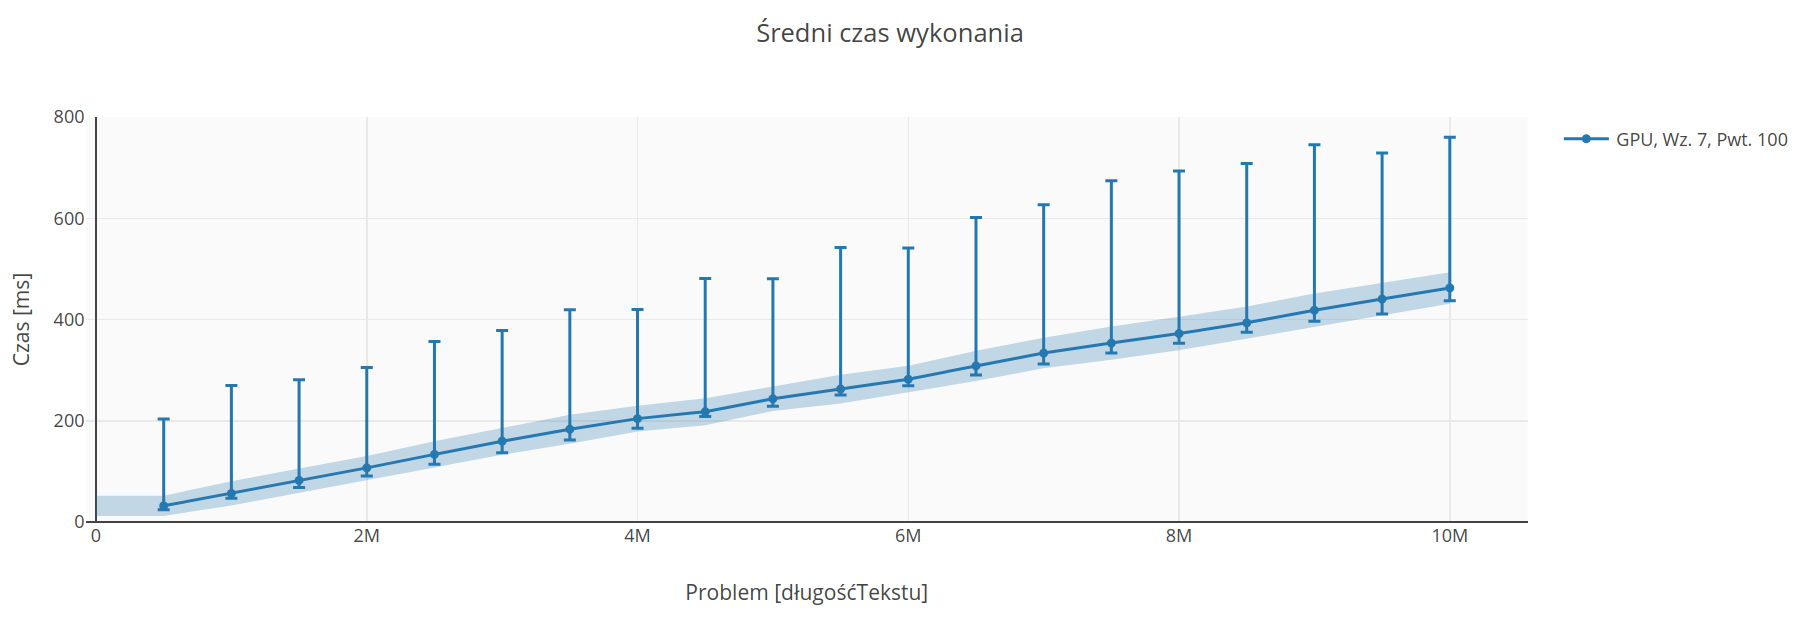
\includegraphics[keepaspectratio, width=1.0\linewidth, trim=0 0 0 2.7cm, clip]{benchmarks/intel_hd520_chrome/gpu_mean.png}
    \caption{Czas wykonania algorytmu GPU, zestaw 2.1}
    \label{fig:chart_gpu_mean_chrome_maja}
\end{figure}

\subsection{Zestawienie}
% rzeczy z~taba w~UI - Podsumowanie

Na rysunkach \ref{fig:chart_summary_chrome_damian} oraz \ref{fig:chart_summary_chrome_maja} zestawiono czasy wykonania algorytmu na CPU oraz GPU. Można zauważyć, iż konfiguracja sprzętowa nie odgrywa tutaj znaczącej roli -- z dokładnością do stałej obie wersje algorytmów mają tą samą charakterystykę czasową niezależnie od platformy sprzętowej.

W przedstawionej skali uwzględniającej średni przypadek wyszukiwania wzorca w tekście można zauważyć, iż wyniki są odwrotne do spodziewanych. Algorytm dla GPU wraz ze wzrostem długości tekstu, liniowo zwiększa czas potrzebny na obliczenie wyniku -- czas jego wykonania jest rządu 100 ms, co może być zauważalne dla użytkownika. Dla CPU sytuacja jest odwrotna; mimo, iż CPU charakteryzuje się obliczeniami sekwencyjnymi, to nawet dla naiwnego wyszukiwania wzorca w tekście można przyjąć, iż czas wykonania algorytmu jest stały w rozważanej skali. Wiadomo z rysunku \ref{fig:chart_cpu_sc_mean_chrome}, że algorytm ten ma w przybliżeniu złożoność liniową, jednak zmiana rzędu 10 ms byłaby niezauważalna dla użytkownika.

Sytuacja ta może wynikać z faktu, iż wraz ze wzrostem rozmiaru problemu (w tym przypadku długości tekstu) wymagane jest przydzielenie kolejnych wątków obliczeniowych na GPU, co zwiększa liczbę danych do późniejszego odczytania z bufora GPU i przekonwertowania do ustalonego formatu. Operacje transferu danych są na GPU kosztowne. W przypadku CPU problem ten nie występuje i pomimo swojej sekwencyjnej natury problem wyszukiwania naiwnego jest przez CPU rozwiązywany znacznie efektywniej.

\begin{figure}
    \centering
    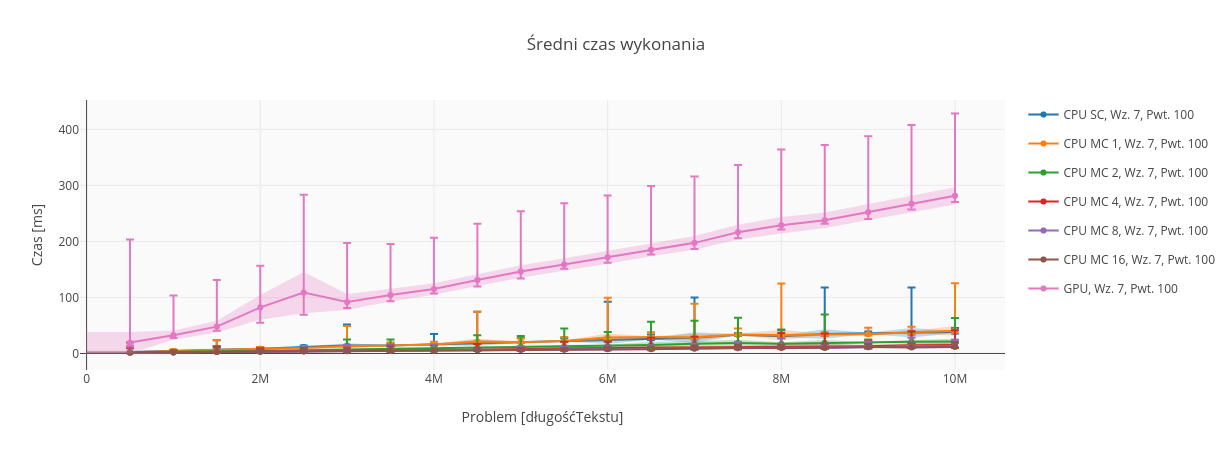
\includegraphics[keepaspectratio, width=1.0\linewidth, trim=1.1cm 0.9cm 0.5cm 3.5cm, clip]{benchmarks/nvidia970_chrome/summary_mean.png}
    \caption{Podsumowanie czasów wykonania algorytmu, zestaw 1.1}
    \label{fig:chart_summary_chrome_damian}
\end{figure}

\begin{figure}
    \centering
    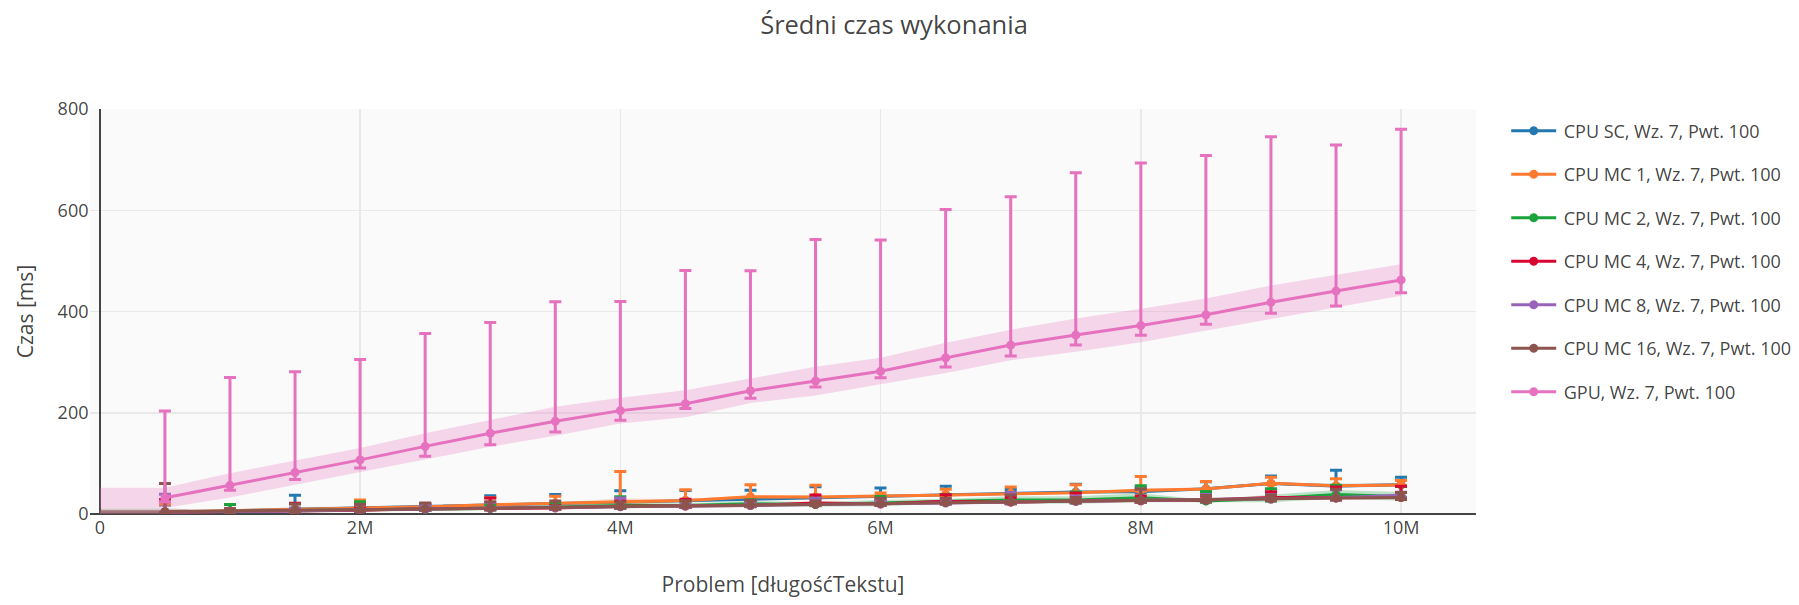
\includegraphics[keepaspectratio, width=1.0\linewidth, trim= 0 0 0 2.7cm, clip]{benchmarks/intel_hd520_chrome/summary_mean.png}
    \caption{Podsumowanie czasów wykonania algorytmu, zestaw 2.1}
    \label{fig:chart_summary_chrome_maja}
\end{figure}
\section{Wnioski i~podsumowanie}
% @everyone - Kuba
% @everyone
% Nie ma co się rozbijać na 100 sekcji

Po wykonaniu badań zaimplementowanych algorytmów można stwierdzić, że akceleracji przy obecnych implementacjach nie udało się uzyskać. Jest to skutkiem zarówno charakterystyki problemu, jak i pośrednika w postaci frameworka GPU.js, które posiada swoje ograniczenia.

Rozwiązaniem, które pomogłoby zwiększyć wydajność analizowanego algorytmu, czyli wariantu ,,brute force'', byłoby rozwiązanie hybrydowe. W~rozwiązaniu takim GPU byłoby odpowiedzialne za sprawdzenie dopasowania wzorca w~tekście dla każdej pozycji. CPU, za pomocą wielu wątków, agregowałby wyniki do oczekiwanej postaci tablicy wystąpień. Akceleracji uległby czas wykonania metody \texttt{filter}, która zajmuje zdecydowaną większość czasu jednego wykonania, co widać na rysunku~\ref{fig:profiler_gpu}. Akceleracja taka będzie efektywna dla dużych rozmiarów problemu, ponieważ w~analizie trzeba wziąć pod uwagę zróżnicowany czas komunikacji z~Workerami.

Do udanych można zaliczyć implementację algorytmu w 3 wariantach, gdyż zaproponowane rozwiązanie jest sprawne. Okazało się, że w odpowiednich warunkach akceleracja może być osiągnięta nawet w środowisku przeglądarki internetowej, które nie podlega kontroli ze strony specjalistycznego oprogramowania -- chociażby operującego na poziomie elementarnych instrukcji GPU środowiska CUDA. Niewątpliwie, wykorzystany framework GPU.js akcelerację umożliwia. Potencjalny stopień akceleracji jest zależny natomiast od rozważanego problemu.

% Citations
\clearpage
\bibliography{bibliography}

\end{document}
